\subsectionaddtolist{الف}

ابتدا کل سیستم را به یک رابطه‌ی فشرده تبدیل می‌کنیم. سیگنال ضربه‌ای میانی برابر است با
\[
x_e(t) = \sum_{n=-\infty}^{\infty} x_d[n]\,\delta(t-nT)
       = K\sum_{n=-\infty}^{\infty} x_b(nT)\,\delta(t-nT)
\]
که همان نمونه‌برداری ضربه‌ای از $x_b(t)$ (با ضریب $K$) است؛ پس در حوزه‌ی فرکانس با تعریف $\omega_s = \frac{2\pi}{T}$:
\[
X_e(\omega) = \frac{K}{T}\sum_{k=-\infty}^{\infty} X_b(\omega - k\omega_s)
\]
فیلتر بازسازی $H(\omega) = T\,\Pi\!\big(\frac{\omega}{2\pi/T}\big)$ یک پایین‌گذر ایده‌آل با بهره‌ی $T$ و فرکانس قطع $\omega_c = \frac{\pi}{T} = \frac{\omega_s}{2}$ است. پس ضریب‌های $T$ و $\frac{1}{T}$ حذف می‌شوند و:
\[
X_f(\omega) = H(\omega)\,X_e(\omega)
           = K\!\!\sum_{k=-\infty}^{\infty} X_b(\omega - k\omega_s)\;\Big|_{\,|\omega|<\omega_s/2}
\]

حال طیف $x_b(t) = x_a(t)\cos(7\pi t)$ از خاصیت مدولاسیون به دست می‌آید:
\[
X_b(\omega) = \frac{1}{2}\big[X_a(\omega-7\pi) + X_a(\omega+7\pi)\big]
\]
چون $X_a(\omega) = \Lambda\!\big(\frac{\omega}{7\pi/2}\big)$ یک مثلث با نیم‌پهنای $\frac{7\pi}{2}$ و قله‌ی $1$ است، $X_b$ دو مثلث در مراکز $\pm 7\pi$ با نیم‌پهنای $\frac{7\pi}{2}$ و قله‌ی $\frac{1}{2}$ خواهد بود (هر مثلث بازه‌ی $[\frac{7\pi}{2}, \frac{21\pi}{2}]$ و قرینه‌ی آن را می‌پوشاند).

با $T=1$ داریم $\omega_s = 2\pi$ و فرکانس قطع $\omega_c = \pi$. رونوشت‌های $X_b$ در گام‌های $2\pi$ تکرار می‌شوند، پس مراکز همه‌ی مثلث‌ها در $\pm 7\pi + 2\pi k$ یعنی روی \emph{همه‌ی مضارب فرد} $\pi$ قرار می‌گیرند:
\[
\text{مراکز مثلث‌ها} = \{\dots, -3\pi,\, -\pi,\, \pi,\, 3\pi,\, 5\pi,\, \dots\}
\]
چون نیم‌پهنای هر مثلث ($\frac{7\pi}{2} = 3.5\pi$) بسیار بزرگ‌تر از $\omega_s = 2\pi$ است، مثلث‌ها به‌شدت هم‌پوشانی دارند. در باند عبور $[-\pi, \pi]$ دقیقا چهار مثلث با مراکز $\{-3\pi, -\pi, \pi, 3\pi\}$ سهم دارند و مقادیرشان جمع می‌شود. با قرار دادن $u = \omega/\pi$ و جمع چهار مثلث:
\[
X_f(\omega) =
\begin{cases}
\dfrac{6}{7}, & |\omega| \leq \dfrac{\pi}{2}\\[10pt]
\dfrac{6}{7} + \dfrac{1}{7}\!\left(\dfrac{|\omega|}{\pi} - \dfrac{1}{2}\right), & \dfrac{\pi}{2} \leq |\omega| \leq \pi\\[10pt]
0, & |\omega| > \pi
\end{cases}
\]
یعنی طیف در میانه تخت و برابر $\frac{6}{7} \approx 0.857$ است و به‌سمت لبه‌ها کمی بالا رفته تا $\frac{13}{14} \approx 0.929$ در $\omega = \pm\pi$ می‌رسد، سپس به‌دلیل فیلتر ایده‌آل به‌طور ناگهانی صفر می‌شود. این طیف در شکل زیر رسم شده است:

\begin{center}
\IfFileExists{figs/2.png}
  {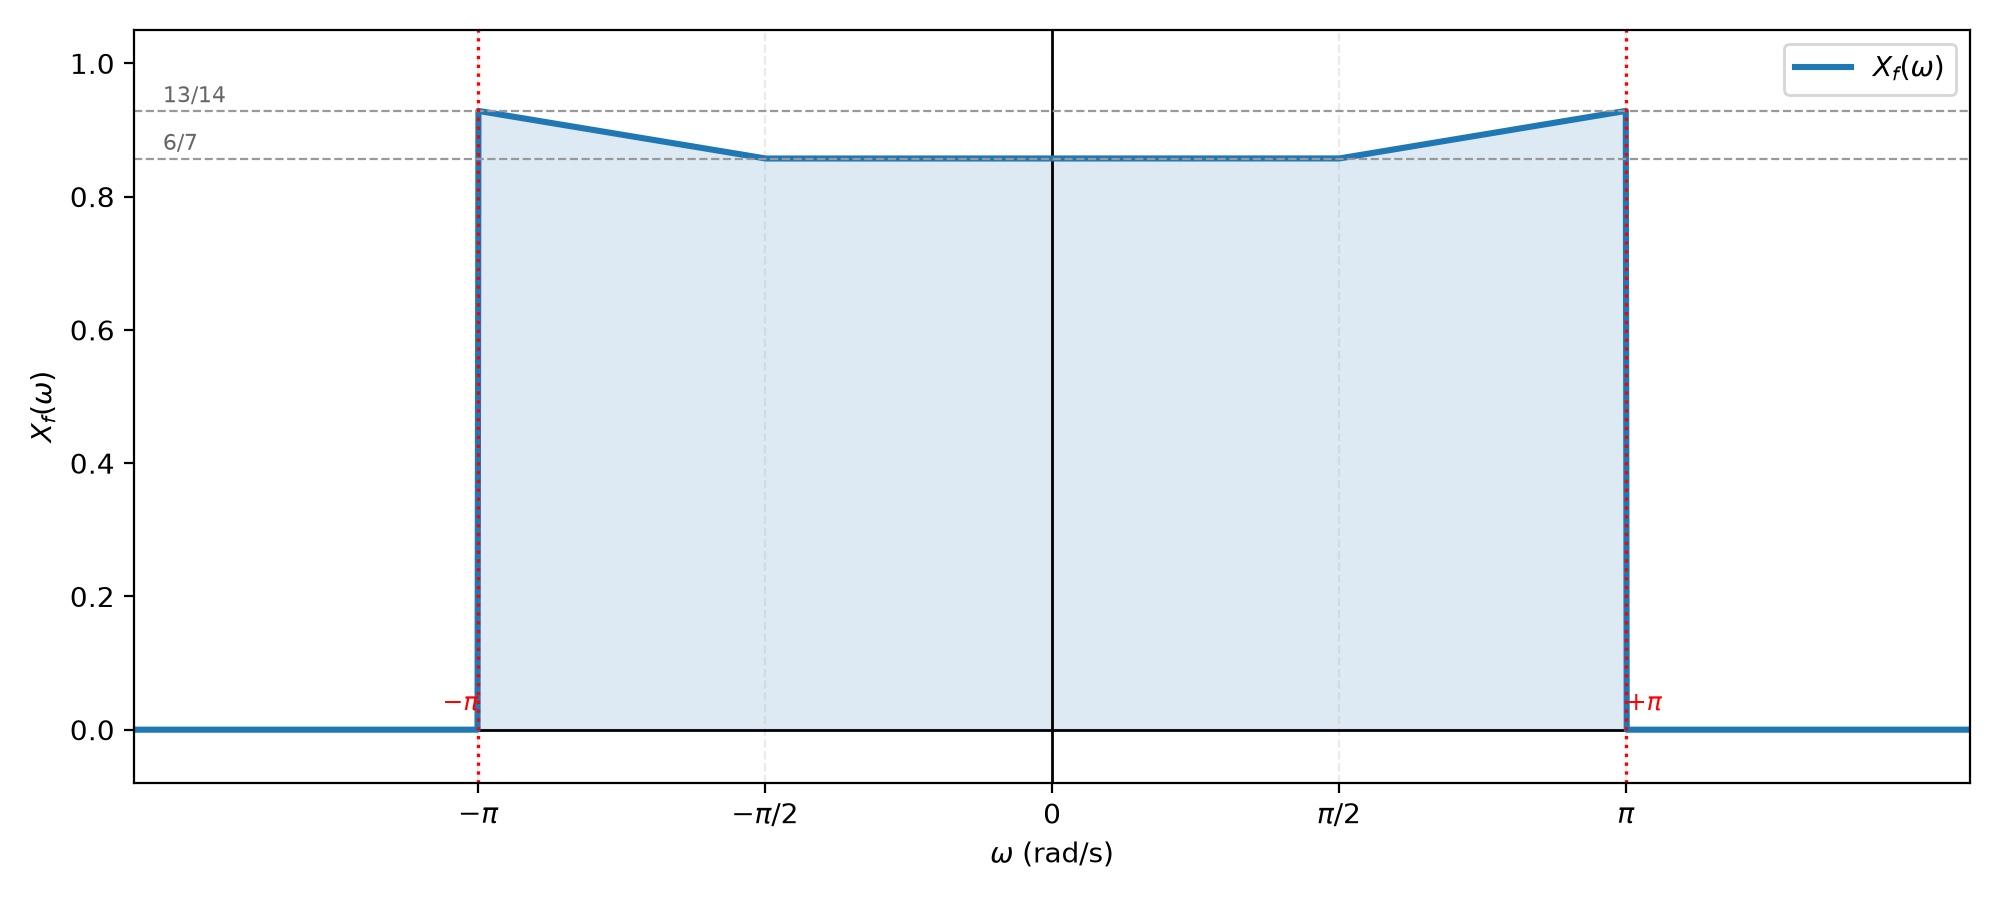
\includegraphics[width=1\textwidth]{figs/2.png}}
  {\fbox{\parbox{0.8\textwidth}{\centering \vspace{2em} «جای نمودار طیف $X_f(\omega)$ — تصویر در \lr{figs/2.png} قرار گیرد» \vspace{2em}}}}
\end{center}

\subsectionaddtolist{ب}

{بله، ممکن است.} برای آنکه خروجی برابر $x_a$ (یک مثلث پایه‌باند) شود، باید یکی از رونوشت‌های $X_b$ دقیقا مرکزش روی مبدأ بیفتد. مرکز مثلث‌ها در $\pm 7\pi + k\omega_s$ است؛ شرط نشستن روی صفر:
\[
k\,\omega_s = 7\pi \quad\Longrightarrow\quad \omega_s = \frac{7\pi}{k},\quad k\in\mathbb{Z}^{+}
\]
اما برای آنکه فیلتر کل مثلث پایه‌باند (نیم‌پهنای $\frac{7\pi}{2}$) را عبور دهد و رونوشت‌های مجاور وارد باند نشوند، لازم است:
\[
\omega_c = \frac{\omega_s}{2} \geq \frac{7\pi}{2}
\quad\Longrightarrow\quad
\omega_s \geq 7\pi
\]
ترکیب دو شرط $\omega_s = \frac{7\pi}{k}$ و $\omega_s \geq 7\pi$ تنها با $k=1$ سازگار است، پس:
\[
\omega_s = 7\pi
\quad\Longrightarrow\quad
T = \frac{2\pi}{\omega_s} = \frac{2\pi}{7\pi} = \frac{2}{7}
\]

با این انتخاب، رونوشت‌های $k = \pm 1$ هر کدام نصف مثلث پایه‌باند را می‌سازند و با هم جمع می‌شوند:
\[
\sum_{k} X_b(\omega - 7\pi k)\Big|_{\text{باند پایه}}
= \frac{1}{2}X_a(\omega) + \frac{1}{2}X_a(\omega) = X_a(\omega)
\]
و مثلث مجاور دقیقا از لبه‌ی $\frac{7\pi}{2}$ (محل قطع فیلتر) شروع می‌شود، پس هیچ هم‌پوشانی‌ای رخ نمی‌دهد. در نهایت:
\[
X_f(\omega) = K\cdot X_a(\omega)
\quad\Longrightarrow\quad
x_f(t) = x_a(t) \iff K = 1
\]

پس تنها مقدار ممکن عبارت است از:
\[
{\,K = 1, \qquad T = \frac{2}{7}\,}
\]

نمونه‌برداری به‌خودی‌خود رونوشت‌هایی از طیف می‌سازد؛ اگر نرخ نمونه‌برداری درست انتخاب شود ($\omega_s = 7\pi$)، یکی از این رونوشت‌ها سیگنال میان‌باند را دقیقا به پایه‌باند منتقل می‌کند و عمل نمونه‌برداری خودش نقش \emph{دمدولاسیون} را ایفا می‌کند و $x_a$ کاملا بازسازی می‌شود. اما با نرخ نامناسب (مثل $T=1$) رونوشت‌ها روی هم می‌افتند و آلیاسینگ، طیف را مخدوش می‌کند. درس مهم این است که نرخ نمونه‌برداری باید با محل و پهنای باند سیگنال هماهنگ باشد، نه صرفا بزرگ بودن آن.
